\documentclass[a4paper,11pt,twoside]{scrartcl}
\usepackage[T1]{fontenc}
\usepackage{subcaption}
\usepackage[utf8]{inputenc}
\usepackage{ngerman, eucal, mathrsfs, amsfonts, bbm, amsmath, amssymb, stmaryrd,graphicx, array, geometry, color, wrapfig, float, hyperref}
\geometry{left=25mm, right=15mm, bottom=25mm}
\setlength{\parindent}{0em} 
\setlength{\headheight}{0em} 
\title{Machine Learning\\ Blatt 8}
\author{Markus Vieth\and David Klopp\and Christian Stricker}
\date{\today}
\usepackage{listings, textcomp}
\usepackage[usenames,dvipsnames,svgnames,table]{xcolor}


\definecolor{Code}{rgb}{0,0,0}
\definecolor{Keywords}{rgb}{0,0,255}
\definecolor{Strings}{rgb}{255,0,0}
\colorlet{Comments}{Green}
\colorlet{Numbers}{blue}

%%%%%%%%%%%
%Mache Integer farbig
%%%%%%%%%%%

\makeatletter

\newif\iffirstchar\firstchartrue
\newif\ifstartedbyadigit

\newcommand\processletter
{%
	\ifnum\lst@mode=\lst@Pmode%
	\iffirstchar%
	\global\startedbyadigitfalse%
	\fi
	\global\firstcharfalse%
	\fi
}

\newcommand\processdigit
{%
	\ifnum\lst@mode=\lst@Pmode%
	\iffirstchar%
	\global\startedbyadigittrue%
	\fi
	\global\firstcharfalse%
	\fi
}

\lst@AddToHook{Output}%
{%
	\ifstartedbyadigit%
	\def\lst@thestyle{\color{Numbers}}%
	\fi
	\global\firstchartrue%
	\global\startedbyadigitfalse%
}

\newtoks\jubo@toks
\jubo@toks={
	language=C,
	commentstyle=\color{Comments}\slshape,
	stringstyle=\color{Strings},
	keywordstyle={\color{Keywords}\bfseries},
	alsoletter=0123456789,
	SelectCharTable=%
}
\def\add@savedef#1#2{%
	\begingroup\lccode`?=#1\relax
	\lowercase{\endgroup
		\edef\@temp{%
			\noexpand\lst@DefSaveDef{\number#1}%
			\expandafter\noexpand\csname lsts@?\endcsname{%
				\expandafter\noexpand\csname lsts@?\endcsname\noexpand#2}%
		}}%
		\jubo@toks=\expandafter{\the\expandafter\jubo@toks\@temp}%
	}
	\count@=`0
	\loop
	\add@savedef\count@\processdigit
	\ifnum\count@<`9
	\advance\count@\@ne
	\repeat
	\count@=`A
	\loop
	\add@savedef\count@\processletter
	\ifnum\count@<`Z
	\advance\count@\@ne
	\repeat
	\count@=`a
	\loop
	\add@savedef\count@\processletter
	\ifnum\count@<`z
	\advance\count@\@ne
	\repeat
	%\showthe\jubo@toks % for debugging
	\begingroup\edef\x{\endgroup
		\noexpand\lstdefinestyle{pseudo}{\the\jubo@toks}
	}\x
	
	\makeatother
%%%%%%%%%%
%Ende
%%%%%%%%%%



\lstset{
	literate={ö}{{\"o}}1
	{ä}{{\"a}}1
	{ü}{{\"u}}1
	{ß}{{\ss}}1
	{/pi}{{$\Pi$}}1
	{/inf}{{$\infty$}}1
	{/eIn}{{$\in$}}1
	{/cup}{{$\cup$}}1
	{/leer}{{$\emptyset$}}1
	{<=}{{$\leq$}}1
	{>=}{{$\geq$}}1
}


\lstset{
	numberstyle=\tiny,
	stepnumber=1,
	numbersep=10pt,
	xleftmargin=15pt,
	breaklines=true,
	numberblanklines=false,
	showstringspaces=false,
	flexiblecolumns=true,
	mathescape=true,
	tabsize=4,
	captionpos=b,
	numbers=left,
	commentstyle=\color{Green},
	numberstyle=\color{gray},
	keywordstyle=\color{blue} \textbf,%otherkeywords={xdata},
	keywords=[2]{xdata},
	keywordstyle=[2]\color{red}\textbf,
	identifierstyle=\color{black},
	stringstyle=\color{red}\ttfamily,
	basicstyle = \ttfamily \color{black} \footnotesize,
	inputencoding=utf8,
	emph=[1]%
	{%
		infinity,
	}, 
	emphstyle=[1]{\color{blue}},
	emph=[2]%
	{%
		forall,
		while,
		if,
		else,
		for,
		return,
		new,
		NULL,
		null,
		int, 
		double, 
		float,
		class,
		void,
		false, 
		true,
		FALSE,
		TRUE,
	}, 
	emphstyle=[2]{\color{Magenta}},
	emph=[3]{b0, b1, n0, n1},
	emphstyle=[3]{\color{black}}
}
\begin{document}

\newcommand{\cor}[1]{\textcolor{red}{\textit{#1}}}
\maketitle
\cleardoublepage
\pagestyle{myheadings}
\markboth{Markus Vieth,  David Klopp, Christian Stricker}{Markus Vieth, David Klopp, Christian Stricker}

\newpage

\section*{Nr. 3.1}
Design a two-input perceptron that implements the boolean function $A \land \neg B$\\

\subsection*{1. Allgemein:} \[w_0 + w_1 \cdot x_1 + w_2 \cdot x_2\]

\subsection*{2. Bedingungen:}

\[\text{I.}~w_0 - w_1 - w_2 \leq 0 \]
\[\text{II.}~w_0 - w_1 + w_2 \leq 0 \]
\[\text{III.}~w_0 + w_1 - w_2 > 0 \]
\[\text{VI.}~w_0 + w_1 + w_2 \leq 0 \]

\subsection*{3. Rechnung:}

\subsubsection*{1. I + VI}
\[2 \cdot w_0 \leq 0 \Leftrightarrow w_0 \leq 0 \]

\subsubsection*{2.}
\[\text{I.} \Leftrightarrow w_0 \leq w_1 + w_2\]
\[\text{III.} \Leftrightarrow w_0 > -w_1 + w_2\]
\[\Rightarrow -w_1 + w_2 <  w_0 \leq w_1 + w_2\]
\[\Rightarrow -w_1 + w_2 < w_1 + w_2\]
\[ \Leftrightarrow w_1 > 0\]

\subsubsection*{3. Wähle $w_0 = 0$ und $w_1 = 1$}

\[ 0 -1 -w_2 \leq 0\]
\[ -1 \leq w_2\]
\subsubsection*{4. Wähle $w_2 = -1$}

\[\text{I.}~0 - 1 +1 = 0 \leq 0~~~\checkmark \]
\[\text{II.}~0 - 1 - 1 = -2 \leq 0~~~\checkmark \]
\[\text{III.}~0 + 1 +1 = 2 > 0~~~\checkmark \]
\[\text{VI.}~0 + 1 -1 = 0 \leq 0~~~\checkmark \]

\subsubsection*{5. Lösung:}
\[
\overset{\rightarrow}{w} = \begin{pmatrix}
           0 \\
           1 \\
           -1
         \end{pmatrix}
\] 

\pagebreak

\section*{Nr. 3.2}
\begin{figure}[H]
\centering
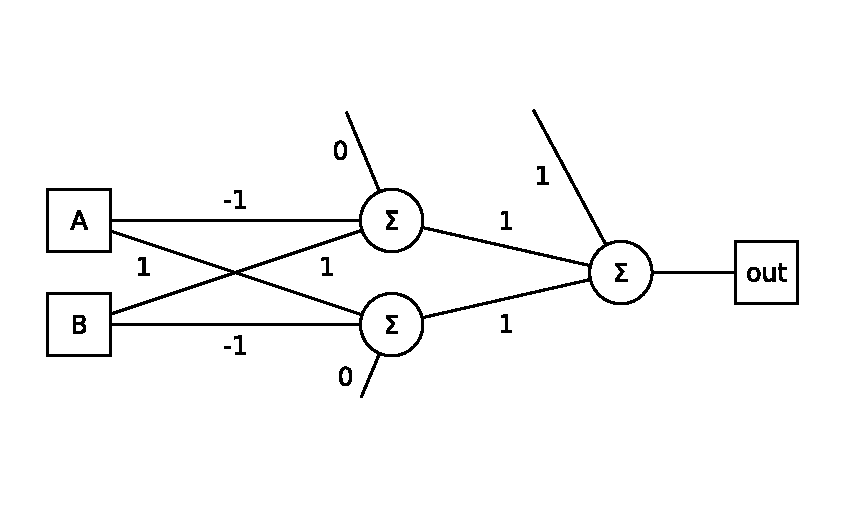
\includegraphics{2Layer}
\caption{Zahlen entsprechen Gewichten, Kanten ins Leere entsprechen $w_0$. Die erste Schicht entspricht der Teilaufgabe 1, zweite Schicht einem Oder $\Rightarrow~~ (A\land\bar{B})\lor(\bar{A}\land B)$}
\label{fig:2Layer}
\end{figure}

\end{document}